%
% begin in Jan. 19th, 2010
%
%
%
%
%%%%%%%%%%%%%%%%%%%%%%%%%%%%%%%%%%%%%%%%%%%%%%%%%%%%%%%%%%%%%%%%%%%%%%
\chapter{Energy Derivatives in Quantum Chemistry}
%
%
%
In quantum chemistry, the evaluating for the energy derivatives with
respect to the changes of system is overwhelming important, for many
aspects; such as energy surface study, the vibration etc. are all have
to employ such technic. Hence in this chapter, we will gather all of
such technics systematically together, and all of content are mainly
from the book written by  Yukio Yamaguchi, John D. Goddard, Yoshihiro
Osamura and Henry
Schaefer\cite{New_Dimension_for_Derivatives_Calculation}. However,
actually many people had made great contribution to this area,
especially Pulay\cite{Pulay1, Pulay2, Pulay3, Pulay4, Pulay5,
Pulay6, pulay:5043}, and other people\cite{bishop:3515,
RevModPhys.45.22, jorgensen:334, king:5645, meyer:2109}. However, the
book by Henry Schaefer etc. is representing a generalization of
nearly all the views or ideas, and the author recommends that
the further reference for each detailed topic can be found in this
book. 


%%%%%%%%%%%%%%%%%%%%%%%%%%%%%%%%%%%%%%%%%%%%%%%%%%%%%%%%%%%%%%%%%%%%%%
\section{Introduction}
In quantum chemsitry, the core idea for approximating general wave
function is called ``single electron approximation'' (in DFT, it's
called non-interacting system mapping relationship). This important
idea introduces the idea of molecular orbital, where the general wave
functions for the whole system is building from it. The relation
between the MO and the general wave function etc. is depicted in the
figure\ref{derivatives_fig:1}.
\begin{figure}[bhtp]
 \centering
 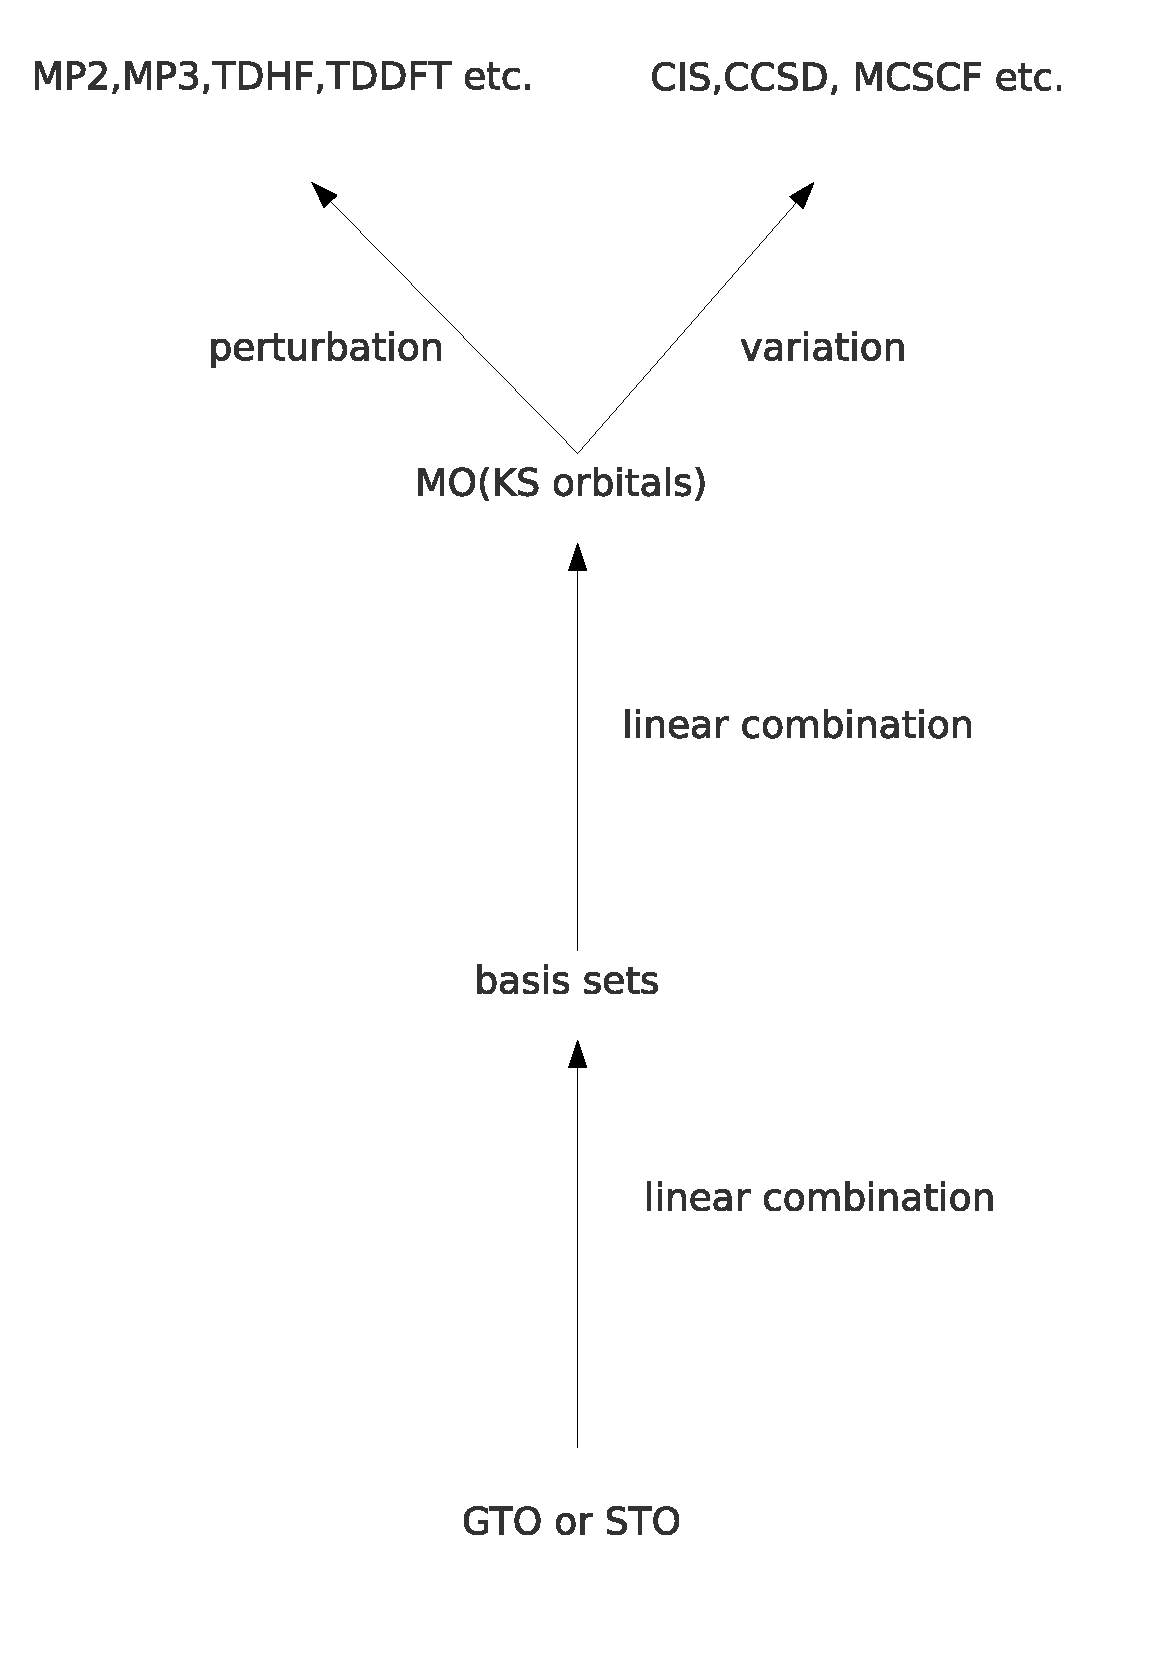
\includegraphics[scale=0.7]{mo_in_energy_drv.eps}
 \caption{MO general description}
 \label{derivatives_fig:1}
\end{figure}

Here as what has been demonstrated in (\ref{derivatives_fig:1}), the
MO is composed by two parts: one is the basis set functions (we can
know it always takes the GTO or STO form, the other form like plane
wave function is rarely used), the other is the MO coefficients
before each basis sets function. Hence, all the energy derivatives
will finally be expressed based on the basis sets function integrals
derivatives and the MO coefficient derivatives. Now in this section
we will give some analysis to this part.

%%%%%%%%%%%%%%%%%%%%%%%%%%%%%%%%%%%%%%%%%%%%%%%%%%%%%%%%%%%%%%%%%%%%%%
\section{Derivatives expressions for the integrals and the MO
coefficients}
%
%
%
%
%%%%%%%%%%%%%%%%%%%%%%%%%%%%%%%%%%%%%%%%%%%%%%%%%%%%%%%%%%%%%%%%%%%%%%
\subsection{General Perturbation method}
%
%
%
The energy derivatives could be considered as a small preturbation on
the Hamiltonian (because of the geometrical changes or the adding on
some electric fields). Just let's take geometrical change as an
example, hence the Hamiltonian can be expressed as some Talor
expansion:
\begin{equation} 
\label{General_Perturbation_method_eq:1}
 \hat{H} =
\hat{H}_{0}+\lambda_{a}\hat{H}_{a}^{'}+\lambda_{b}\hat{H}_{b}^{'} + 
\frac{1}{2}\lambda_{a}^{2}\hat{H}_{a}^{''} +
\frac{1}{2}\lambda_{b}^{2}\hat{H}_{b}^{''} + 
\lambda_{a}\lambda_{b}\hat{H}_{ab}^{''}    + \cdots
\end{equation}
Here the $\lambda$ character the order of perturbation (similar with
the $\lambda$ in the \ref{PTIQMeq:1}, but as an extension), and the
$\hat{H}^{'}$ and $\hat{H}_{a}^{''}$ are the perturbed operators for
Hamiltonian, $a$ and $b$ characterize different direction for the
geometrical perturbation.

Then according to the perturbation theory, the integrals as well as
the the MO coefficients are all able to expressed in terms of
perturbation series:
\begin{equation} 
\label{General_Perturbation_method_eq:2}
 S_{\mu\nu}^{perturbed} =
S_{\mu\nu}+
\lambda_{a}\frac{\partial S_{\mu\nu}}{\partial a} + 
\lambda_{b}\frac{\partial S_{\mu\nu}}{\partial b} +
\frac{1}{2}\lambda_{a}^{2}
\frac{\partial^{2} S_{\mu\nu}}{\partial a^{2}} + 
\frac{1}{2}\lambda_{b}^{2}
\frac{\partial^{2} S_{\mu\nu}}{\partial b^{2}} +
\lambda_{a}\lambda_{b}
\frac{\partial^{2} S_{\mu\nu}}{\partial a\partial b} +
\cdots
\end{equation}
This is for the overlap integrals in AO. For the MO coefficients, the
expression is same:
\begin{equation} 
\label{General_Perturbation_method_eq:3}
 C_{i}^{perturbed} =
C_{i}+
\lambda_{a}\frac{\partial C_{i}}{\partial a} + 
\lambda_{b}\frac{\partial C_{i}}{\partial b} +
\frac{1}{2}\lambda_{a}^{2}
\frac{\partial^{2} C_{i}}{\partial a^{2}} + 
\frac{1}{2}\lambda_{b}^{2}
\frac{\partial^{2} C_{i}}{\partial b^{2}} +
\lambda_{a}\lambda_{b}
\frac{\partial^{2} C_{i}}{\partial a\partial b} +
\cdots
\end{equation}
This is the starting point for further study. 


%%%%%%%%%%%%%%%%%%%%%%%%%%%%%%%%%%%%%%%%%%%%%%%%%%%%%%%%%%%%%%%%%%%%%%


%%% Local Variables: 
%%% mode: latex
%%% TeX-master: "../../main"
%%% End: 
